%%=============================================================================
%% Methodologie
%%=============================================================================

\chapter{\IfLanguageName{dutch}{Methodologie}{Methodology}}
\label{ch:methodologie}

\section{Inleiding}
Om een antwoord te krijgen op de onderzoeksvraag wordt er een experiment opgesteld. Dit experiment zal per benadering van de verschillende State Management twee resultaten opleveren. Het eerste resultaat zal het aantal lijnen code van het project bevatten. Hoe deze meting te werk zal gaan wordt in de volgende sectie besproken. Als tweede resultaat wordt een automatische procedure een aantal keer doorlopen, dit wordt uitvoeriger besproken in \ref{se:prestaties}.

Als eerst worden de nodige voorbereidingen voor dit experiment besproken.

\section{Voorbereidingen}
De layout van de mobiele applicatie is gebasseerd op een mock-up. Deze mock-up werd vooraf gemaakt zodat er tijdens het ontwikkelen van de initiële broncode geen tijd verloren gaat. De mock-ups zijn onder deze sectie terug te vinden.

De applicatie heet StoreIt, het hoofddoel van de applicatie is om producten op te lijsten en producten toe te voegen als verkoper. Om de complexiteit van de app te beperken wordt er geen onderscheid gemaakt voor \textit{een klant} en \textit{een verkoper}. De koper heeft als doel de producten lijst te raadplegen en de details van een product te bekijken. Een verkoper heeft als hoofddoel om een product toe te voegen. In dit experiment worden de klant en de verkoper als een beschouwd. Er is ook nog een mogelijkheid om op het voorkeuren scherm het thema van de applicatie in te stellen. De beschikbare thema's zijn lichte- en donkere modus.
De \textbf{bottom navigation bar} zal ervoor zorgen dat de verschillende schermen worden getoond op de juiste tab. Voor het veranderen van de tab wordt een index bijgehouden om te weten welke tab actief is. Hiervoor wordt \verb|setState()| gebruikt, aangezien er sprake is van een ephemeral state.

De focus van de verschillende benaderingen van State Management worden toegepast op volgende zaken: 
\begin{itemize}
    \item De gebruiker wijzigt het thema op het Voorkeuren scherm.
    \item De gebruiker voegt een nieuw product toe, als gevolg dat de lijst van producten moet bijgewerkt worden op de andere tab.
    \item De gebruiker verwijdert een product op het Product Details scherm, als gevolg dat de lijst van producten moet bijgewerkt worden op de andere tab.
\end{itemize}
Voor deze puntjes zal per benadering te broncode worden aangepast. De broncode van eenbenadering van een State Management wordt gestart vanaf de boiler template code. Deze template wordt op voorhand geschreven. Deze code bevat onder andere de nodige widgets, bijvoorbeeld een product-item, de knoppen...
Bij deze template is geen sprake van State Management, buiten de state van de \verb|BottomNavigationBar|, dit wordt aangevuld per verschillende benadering.

\begin{figure}
    \begin{tabular}{cc}
        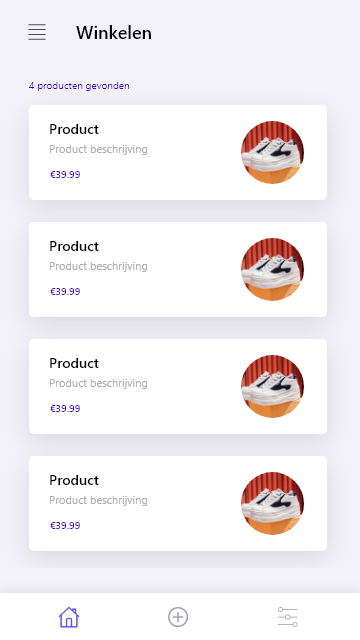
\includegraphics[width=65mm]{img/methodologie/mock-home_screen.png} &   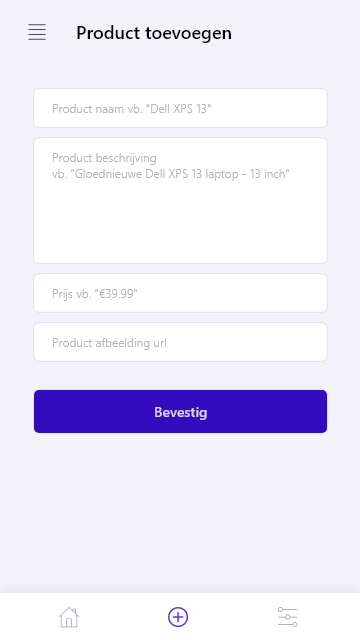
\includegraphics[width=65mm]{img/methodologie/mock-add_product_screen.png} \\
        (a) Mock-up: product lijst scherm & (b) Mock-up: product toevoegen scherm\\[6pt]
        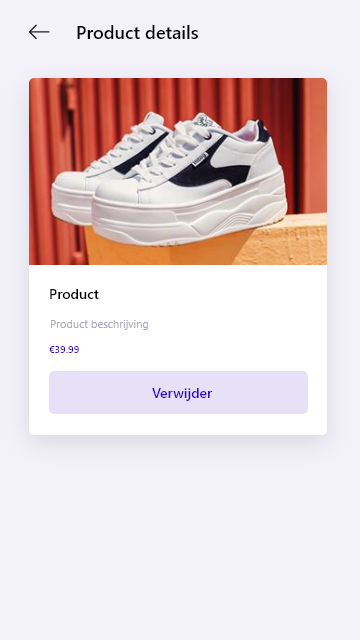
\includegraphics[width=65mm]{img/methodologie/mock-details_screen.png} &   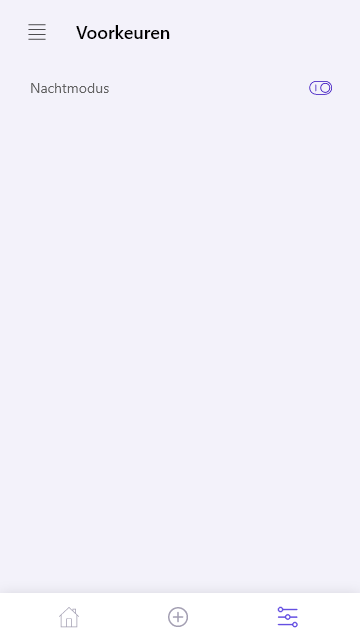
\includegraphics[width=65mm]{img/methodologie/mock-preferences.png} \\
        (c) Mock-up: product details scherm & (d) Mock-up: Voorkeuren scherm \\[6pt]
    \end{tabular}
    \caption{caption}
\end{figure}

\section{Aantal lijnen code}
Om een benaderend meetniveau te verkrijgen voor de complexiteit van een State Management worden de aantal lijnen code geteld. Dit resultaat zal een beeld scheppen op de hoeveelheid code moet geschreven worden om een benadering van State Management uit te schrijven. Merk op dat de complexiteit verschillend is van ontwikkelaar tot ontwikkelaar, dit is en blijft een subjectief meetniveau. Uit dit resultaat wordt besloten hoe rap een benadering van State Management geschreven kan worden. Dit kan leiden tot bijvoorbeeld volgende conclusies: Flutter beginners zullen de voorkeur geven aan benaderingen die rapper zijn te schrijven. 

De aantal lijnen code van de Dart bestanden worden geteld, dit zijn de bestanden met de \verb|.dart| extensie. Hiervoor wordt per verschillende benadering het volgende commando gebruikt: \verb|find . -name '*.cs' | xargs wc -l|. Dit commando geeft het totaal aantal lijnen terug, dit zal per verschillende benadering uitgevoerd worden. Tijdens het schrijven van de benaderingen wordt er rekening gehouden met volgende afspraken: commentaar in de code wordt, vooraleer het commando wordt uitgevoerd, verwijderd. Er wordt enkel gebruik gemaakt van een backspace (nieuwe lijn) voor de scheiding van de verschillende methodes.

\section{Prestaties}
\label{se:prestaties}

%% TODO: Hoe ben je te werk gegaan? Verdeel je onderzoek in grote fasen, en
%% licht in elke fase toe welke stappen je gevolgd hebt. Verantwoord waarom je
%% op deze manier te werk gegaan bent. Je moet kunnen aantonen dat je de best
%% mogelijke manier toegepast hebt om een antwoord te vinden op de
%% onderzoeksvraag.

\lipsum[21-25]

